\section{A Quantitative Metric to \\ Evaluate Security Feature \\ of the Kernel}
\label{sec.metric}
In this section, we first discuss the reasons for us to come up with our metric. 
We then describe what our metric is. To use our metric, we have a key hypothesis that 
commonly used kernel paths are likely to contain fewer bugs. This hypothesis, if verified, 
could be leveraged to create new designs for building secure systems. We did experiments 
to try to verify our hypothesis. We demonstrate that our hypothesis is indeed true by showing 
the data and results we obtained using our metric. We also discussed more general use of 
our metric (in designs with goals other than building secure systems \yiwen{this can be changed 
if we want to emphasize security. We can instead talk about achieving a tradeoff between security 
and functionality}).
In the following section, we introduce a new design that only places limited trust within 
the commonly used kernel paths, as an example of using our metric to create designs 
for secure systems.

\subsection{Why Do We Need the Metric?}
As discussed in the previous section \S{2}, a key reason that existing techniques 
fail to provide strong protection to the kernel is that there has yet to be a good way 
or standard method to understand which portion of the kernel is safe 
and which portion of the kernel is risky. We need to gain more knowledge about 
this question to properly decide how should the kernel be exposed to the user applications, 
and what could be the best way to protect interactions between the kernel space and 
the user space, without drastic change of the 
current kernel structure. Thus, a metric to help solve this problem is desirable 
and could have huge practical impact. 

In addition to having a standard method for measuring and evaluating the kernel, 
our metric would also become a solid basis to conduct comparison between different systems. 
Surprisingly, researchers and developers did not have a good way to evaluate the security feature 
of their systems, let along conduct comparison between different systems. However, to achieve the 
goal of building and deploying secure systems, it is critical that our community put our efforts together 
and improve our work based upon other people's work. Therefore, doing fair and accurate comparison 
between different systems becomes very important. And our metric provides a quantitative way to 
facilitate such comparison. We conducted and show such comparison between different systems in 
our evaluation section. 

\subsection{Our Metric and the Key Hypothesis}
The Operating System kernel source code is organized under different kernel paths and folders. 
Whenever system resources, such as I/O, memory, and CPU, need to be accessed, the kernel code 
under corresponding paths will be executed to perform necessary functions. Therefore, the kernel code 
execution can be viewed as the fundamental activities of the kernel, and it reflects the basic behavior of 
the kernel. Thus, it makes sense to measure and analyze which lines of code get executed in the kernel. 
Our metric adopts this fundamental approach. It first captures which lines of code in the kernel get executed 
when running certain task programs, which we called \textbf{\textit{the kernel trace}}. The kernel trace closely
ties with the set of task programs that generated the trace. Therefore, conducting comparison between 
different environments and systems becomes possible, using the kernel traces. To capture the kernel trace, 
we used a tool called Gcov \yiwen{cite: Gcov}, which is a component inside the Linux kernel.

Moreover, our metric makes security evaluation of the kernel code possible. Using historical kernel vulnerability 
reports, we built a list of severe kernel bugs. For each of the bug we examined, we identified the lines of code 
in the kernel that would trigger the bug. We assume that the lines of code in the kernel are \textit{risky} if they 
can trigger certain kernel vulnerabilities. And those lines of code that cannot trigger kernel vulnerabilities are 
considered to be \textit{safe}. This gives us a way to determine which lines of code in the kernel are risky, and 
which lines of code in the kernel are safe.  

Now, to address the problem that motivated our metric from the very beginning, which portions of the kernel 
are safe and which portions of the kernel are risky. We can use our metric to answer this question. To be more
specific, we use our metric to get an idea of which lines of code in the kernel contain fewer bugs, then label 
those lines as safe lines. The safe lines of code would then compose the safe portion of the kernel, which can 
be trusted to build a secure trusted computing base for designs of secure systems (which will be shown in 
section \S 4). 

We have a key hypothesis about which portions of the kernel are safe and contain fewer bugs. The hypothesis 
is, commonly used kernel paths are likely to be safe and contain fewer bugs. Here, ``commonly used kernel paths'' 
means the kernel paths executed by running popular and daily-used applications, such as Web browser applications, 
and file editor applications. The logic behind our hypothesis is that commonly used kernel paths are used frequently 
on a daily basis, and therefore should be well examined and reinforced. In addition, commonly used kernel paths 
are usually kernel functions used in a normal way rather than special corner cases, which means that the chance 
to harbor kernel bugs in those commonly used kernel paths is slim. 

If our hypothesis can be verified, then it would become a critical guideline to create new designs of secure systems 
(shown in section \S 4). 
But before going too far into the new designs, let us first verify that our hypothesis indeed holds, that commonly used
kernel paths are likely to contain fewer bugs and be safer. We verified our hypothesis and present our results 
in the following subsection.

\subsection{Verification of the Key Hypothesis}
To verify our key hypothesis, we first generated commonly used kernel trace by running a set of common tasks. 
We first define ``common tasks'' used to generate the commonly used kernel trace. 

We then examined a list of 40 severe Linux kernel bugs from the last five years. 
We used the list of 40 kernel bugs to check if there are vulnerabilities lie within the kernel trace we obtained. 
Here is the result of our experiment. \yiwen{Here goes a Table or Diagram for the result.}
From this result, we can see that commonly used kernel paths contain fewer bugs, so our hypothesis is true. 
The hypothesis we just verified can help create new designs of secure systems, we will discuss details of the new 
designs in the next section, \S 4.

\subsection{More General Use of Our Metric}
First of all, the metric provides a standard method to conduct quantitative measurement of the kernel traces 
generated when running applications. Although our initial goal of creating the metric is to provide insights into 
the security issues about how to expose the kernel in a safe way. However, the metric itself has more general
benefits and is not specific to security issues. As we can see through our analysis in the following two subsections
\S{3.3.1} and \S{3.3.2}, it is not just a security metric.

\subsubsection{Obtain The Kernel Profiling Data}
To gain insights about how to protect the interaction between the kernel space and the user space, 
we first need to gain basic insights into what the interaction looks like, in a precise and scientific way. 
We used our metric to perform quantitative measurement of the kernel traces by 
running applications under Native Linux. 

First, we are interested in gaining a broad picture of the kernel traces. 
What's the reachable coverage of the kernel traces. 
Here, we took two different approaches to generate the kernel traces. 

User space applications interact with the kernel space essentially through the system call API. 
So all those system calls are at the bottom level, while the applications sit at the top level. 
It makes sense then to profile the kernel traces from both of those two different levels. 
We used two different approaches to obtain the kernel profiling data. 

\textbf{1) the bottom-up approach: run system call fuzzing.}
System call fuzzing is basically running system calls exhaustively with all possible 
arguments and options. We conducted system call fuzzing over more than 300 available system calls, 
which gave us a thorough kernel trace. 

\textbf{2) the top-down approach: run popular user applications.} 
We ran applications that are commonly used by many users on a daily basis, such as web browser application
and file editor application.  

\begin{table}[ht]
\centering
\begin{tabular}{|l|c|}
  \hline
  Approach & kernel coverage (percentage) \\
  \hline \hline
  System Call Fuzzing & 23\% \\
  \hline
  User Applications & 19\% \\
  \hline
\end{tabular}
\caption {Kernel Coverage}
\label{table:kernel_coverage}
\end{table}

\begin{figure}[h]
\centering
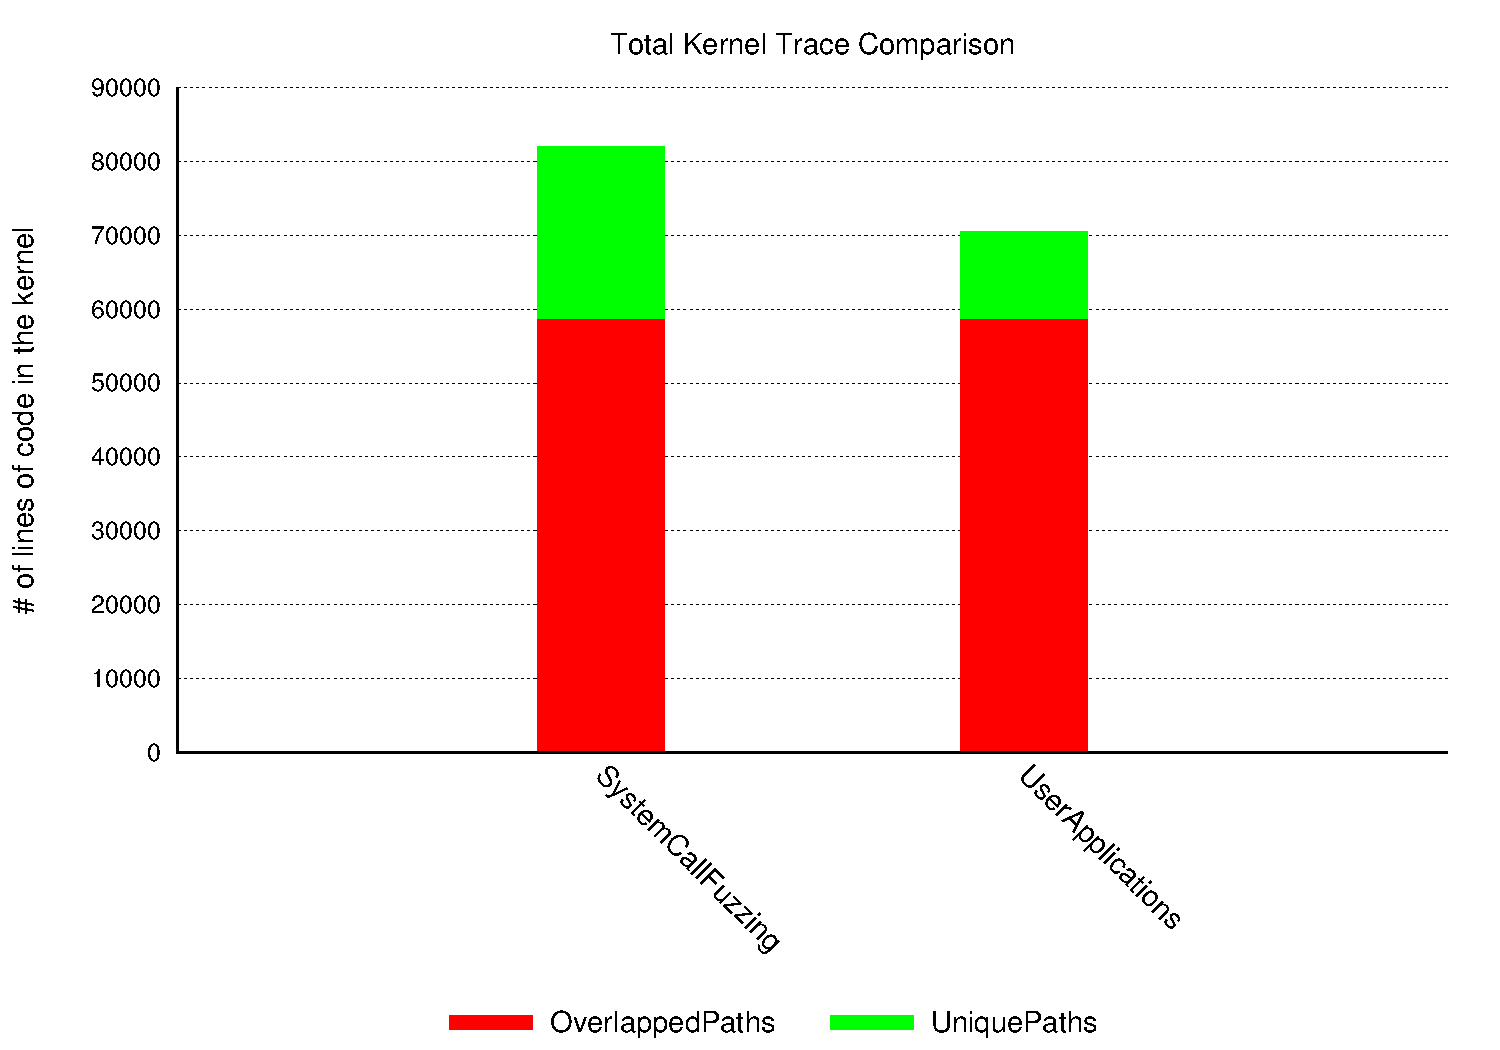
\includegraphics[width=1.0\columnwidth]{diagram/lind_ccs15_diagram_01.pdf}
\caption{Kernel Trace Comparison: Two Approaches}
\label{fig:two_approaches_trace}
\end{figure}

Using the two approaches we just described, we obtained the kernel profiling data.
The kernel trace coverage of the two approaches are as shown in Table 1. 
And further breakdown of the composition of the kernel trace is illustrated in Figure 1.

Among all the kernel trace that were triggered, there were paths in the kernel that 
are vital to managing basic resources, such as I/O, memory, and network. Our kernel profiling data
gave us a chance to see what the kernel trace coverage looked like in those key kernel paths, 
as is shown in Figure 2.

\begin{figure}[h]
\centering
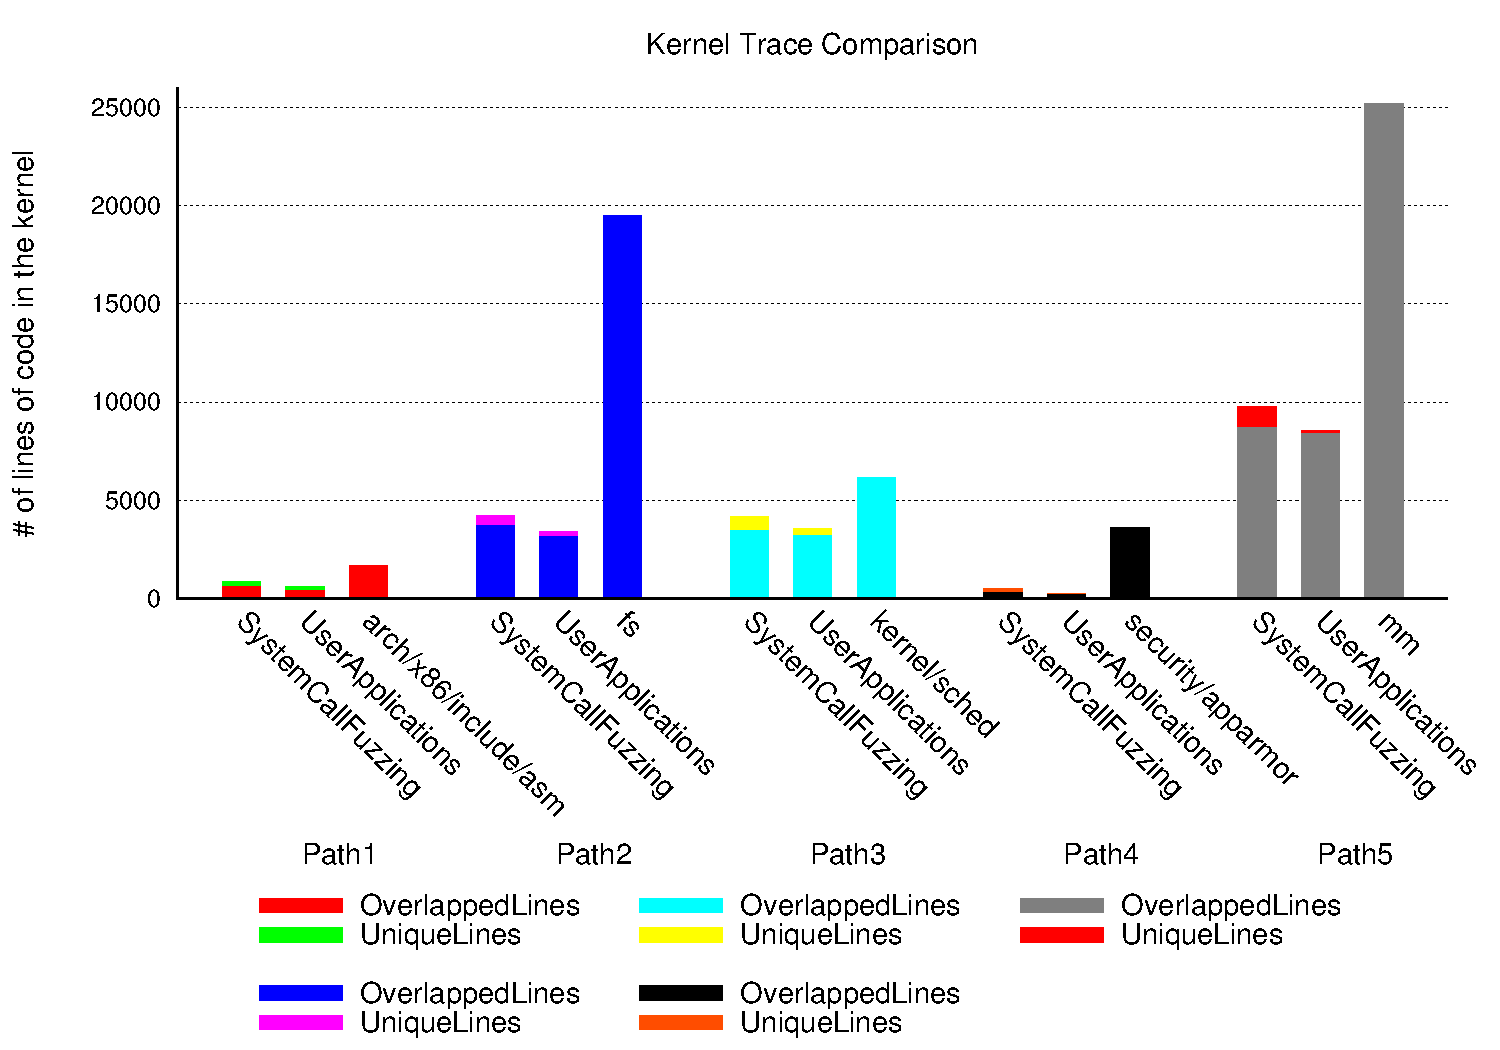
\includegraphics[width=1.0\columnwidth]{diagram/lind_ccs15_diagram_02.pdf}
\caption{Kernel Trace in Key Paths}
\label{fig:key_paths_trace}
\end{figure}

Another way to interpret the kernel profiling data is to look at how many times certain parts of the kernel
have been executed. This can be useful to determine the value of the kernel codes. More frequently executed
code is more likely to impact the functionality and performance of the running programs that triggered the code.
We analyzed the kernel trace frequency for five key kernel path under Native Linux and VirtualBox. The results are 
shown in Figure 3.

\begin{figure}[h]
\centering
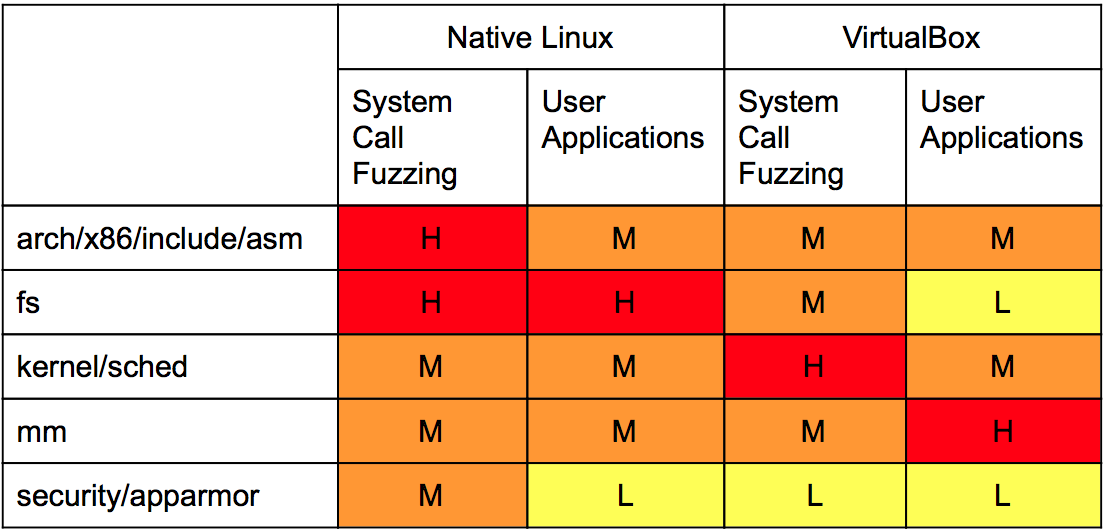
\includegraphics[width=1.0\columnwidth]{diagram/trace_frequency_heatmap.png}
\caption{Kernel Trace Frequency Heatmap. (H: high use frequency, code triggered >= 100 times; 
M: medium use frequency, 20 times <= code triggered < 100 times; L: low use frequency, code triggered < 20 times.)}
\label{fig:trace_frequency_heatmap}
\end{figure}

The above is an example of how to use our metric to obtain information about use frequency of certain kernel paths, 
which could help understand which parts of the kernel is frequently used and therefore very important to 
certain user patterns.

Based upon the use frequency data of the kernel trace, system call interface can also be evaluated using this data. 
System calls that contain more frequently used kernel code are considered more frequently used system calls. 
This information helps determine the importance of system calls and provides a basic guideline 
to help with designs using system call interface.

\subsubsection{How to Use the Kernel Profiling Data?}

The kernel profiling data obtained  by running specific dataset serves as a set of guidelines towards new designs 
with different purposes and focuses. With our metric, we can evaluate the kernel according to different features 
and aspects. For example, we can use frequency to determine the value of different parts of the kernel. Or use 
bug analysis to determine the safety of different parts of the kernel. Moreover, we now have solid ground to judge 
trade-off questions, like how to choose between value and safety. With data obtained through our metric, now, 
we know exactly what kind of tradeoff we are making and what we can get and what we will lose. 

New architecture design can be drawn from guidelines provided by our metric. 
New architecture design might aim at strong secure system (security fist), or full and rich functionality system 
(function first), or fast system (performance first). For each design with specific goal and requirements, look at the
features that are relevant in our metric, and use them as guidelines towards your new design. 
    
Other design issues and concerns may also benefit from using our metric. For example, people may fight between
the idea of kernel space API redesign and the idea of building an user space sandbox to access the existing API. 
Or if we want to build a user space sandbox, what is the best way to design the interface interact with the kernel space.
With our metric, now we have a standard method to obtain kernel profiling data, and make our decisions based upon 
real data and facts.